\chapter{These Millionaires Gave Us Life Changing Advice}

What follows is a chapter built from motion, surprise, and repeated questioning rather than from a single announced thesis. James begins with a day plan, not a theorem: move through Austin, meet successful people, ask sharp questions, and see what survives repetition. Out of that fieldwork a structure gradually emerges. First we are given a clean rule for brand-building. Then that rule is tested against street-level advice about honesty, communication, savings, and debt. Finally the pace slows into a longer conversation with Lavon Perrin, and there the lecture reaches its clearest quantitative comparison: why a policy that looks cheaper each month need not be cheaper over a long horizon.

\section{Opening Setup: The Day as Inquiry}

James frames the day as a sequence of public encounters: get some food, go around downtown Austin, interview wealthy operators, and later continue the work at night. The opening is important because it tells us what kind of notes we are writing. We are not entering a classroom where the proposition is already on the board. We are entering a moving inquiry in which one question opens the next.

That is why the early rhythm is so quick. We pass through music, movement, introductions, and abrupt scene changes before any stable principle is named. The lecture wants to earn its generalizations by repeated contact with actual people. We should therefore let the chapter unfold in that same order: discovery first, abstraction second.

\section{Consumer First: The Nike Case}

A casual question about work history suddenly produces a striking answer. Elliot Hill says that he worked for Nike, and then, a moment later, that he was ultimately president of the company. The surprise matters. It creates the authority for what follows, but it also does something subtler: it sharpens James's next question. Now that the speaker is no longer merely interesting but genuinely consequential, we want to know what principle governed the success.

Hill's answer is the first durable mechanism in the lecture. If we want to build a business, we begin with a strong focus on the consumer. The question is not simply whether we admire the product or the brand. The question is: who are we trying to serve, what problems are we solving for them, and what are we building on the basis of those problems?

The Nike explanation is especially clean because it comes in a sequence. In that sequence Nike served athletes, listened to athletes, converted those insights into innovative products, and then told emotional stories that tied the consumer to the brand and the product. One useful way to compress the logic is this:

\begin{figure}
\centering
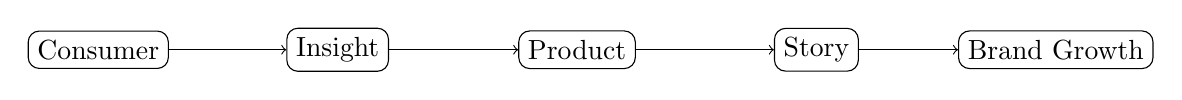
\begin{tikzpicture}[scale=0.95]
\node[draw, rounded corners] (c) at (0,0) {Consumer};
\node[draw, rounded corners] (i) at (3.2,0) {Insight};
\node[draw, rounded corners] (p) at (6.4,0) {Product};
\node[draw, rounded corners] (s) at (9.6,0) {Story};
\node[draw, rounded corners] (b) at (12.8,0) {Brand Growth};
\draw[->] (c) -- (i);
\draw[->] (i) -- (p);
\draw[->] (p) -- (s);
\draw[->] (s) -- (b);
\end{tikzpicture}
\end{figure}

The point of the diagram is not to over-formalize an interview. It is to keep us from reducing the advice to a slogan. Consumer attention has to pass through a sequence of transformations. It must become insight, then product, then narrative. Only after that do we begin to understand why the brand grows.

James then pivots to sales, and the second rule fits naturally beside the first. Many people are afraid to ask. Hill's reply is that one has to be bold, confident, and willing to ask directly for the order. So the opening case produces a compact pair of principles: start from the consumer, and do not hide from the moment of sale.

\section{From the Elite Case to the Street-Level Test}

James does not let the Nike encounter stand alone as a glamorous anecdote. He steps back into narration, remarks on the surprise of having run into the former president of Nike, and then returns to downtown Austin to ask others what has made them successful. This is an important structural move. The lecture is checking whether the same principles survive outside a single high-status example.

The next cluster of answers revolves around self-command. One finance professional answers the question of financial freedom with honesty and transparency, especially honesty with oneself. Social media enters as a kind of epistemic distortion. If we are always reacting to what others appear to be doing, we lose contact with the actual state of our own goals.

From there James asks about skill, and the reply is communication. That answer is deliberately broad. Communication is not treated as a narrow trick for sales or negotiation alone. It is treated as a general commercial faculty: get out of the comfort zone, talk to people, be open, and stop letting hesitation function as a permanent barrier between oneself and opportunity.

The college-degree question then emerges as a natural continuation of the same theme. The answer is not dogmatically anti-college. Rather, the lecture breaks the matter into cases. Some professions structurally require formal schooling. But success in the broader commercial world is not presented as something guaranteed or denied by a credential. Once again the lecture prefers fit over prestige. We ask what the path demands, not what looks socially elevated from the outside.

\section{Early Money Habits: Saving, Debt, and the Cost of Idle Cash}

At this point the lecture tightens around money habits. One interviewee says that marketing is a great skill to have. Another answers the question of financial freedom more concretely: invest, save \(10\%\) to \(15\%\) of each paycheck, and pay down debt first. The advice is simple, but it is already quantitative.

Let \(p\) denote one paycheck and let \(s\) denote the savings rate. The transcript supplies a practical rule:
\begin{equation}
S = s\,p, \qquad 0.10 \le s \le 0.15.
\end{equation}
Here \(S\) is the amount deliberately extracted from the paycheck before consumption absorbs it. At the most elementary bookkeeping level, if this happens over \(n\) paychecks with no further structure imposed, then
\begin{equation}
A_n = nS = ns\,p.
\end{equation}
This is not a theory of wealth. It is the lecture's way of insisting that a savings decision must become a repeated rule rather than an occasional intention.

The next question pushes the point further by asking what one would tell one's younger self. One reply is especially concrete: invest earlier in real estate and stocks, and do less of the thing that looks harmless in the moment, namely leaving money in cash or spending it too casually on trips and incidental pleasures.

We should notice the balance here. The lecture does not deny that youth should contain enjoyment. It says something more disciplined. We can have a good time and still set targets. What must be resisted is not enjoyment as such, but drift. Cash that is never given a destination becomes vulnerable to convenience. That is the practical meaning of the warning against idle cash.

So the structure of the section is now clear. Communication gets us out of our own way socially; savings and debt discipline keep us from getting in our own way financially.

\section{Lavon Perrin: The Lecture Slows Down}

The next pivot changes the tempo of the chapter. James stops collecting short answers and is recognized by a man who says, in effect, that he has seen this before and would be willing to sit down and talk for real. The quick montage gives way to a longer conversation. The lecture now wants to do something more deliberate than gather isolated tips.

Before Lavon Perrin's full business story begins, the conversation briefly turns to Austin itself. James asks what made Austin such a capital for growth in technology and business, and the answer emphasizes a laid-back atmosphere and a more authentic style of life. That observation matters because it gives the surrounding city a role. Austin is not only where the interviews happen; it is itself presented as a business environment shaped by openness and informality.

James is then taken to what he describes as one of the coolest apartments he has seen in Austin. The spectacular setting is part of the narrative rhythm. It gives visible shape to the aspiration that many younger viewers have, and it prepares the lecture to ask not just how one makes money, but how one organizes a life that makes such outcomes possible.

Lavon is introduced with an additional quantitative credential: James reports that a prior interview with him drew \(2.3\) million views, \(3{,}000\) comments, \(30{,}000\) saves, \(70{,}000\) shares, and over \(1\) million views on Twitter. These numbers do not prove the truth of his advice, but they justify why the lecture now lingers.

Lavon's own story comes in stages. He starts with MCI, when long-distance calling was itself a commercial object. He succeeds there, becomes one of the youngest supervisors, then moves through his own business and private driving for celebrities. COVID then arrives as a shock. The lecture sharpens at exactly that point, because now we have a genuine decision problem: return to insurance, or move more fully into real estate, which was booming at the time.

Lavon's answer is not a single heroic leap. He returns to insurance and then, through insurance, reconnects with real estate. This is one of the clearest pieces of business reasoning in the lecture. We do not always move into a desired field by a direct line. Sometimes we re-enter through an adjacent line of work that restores cash flow, relationships, and momentum.

That is why his later remark matters so much: he is in business for himself, but not by himself. The lecture is quietly replacing the myth of total autonomy with a more accurate picture of commercial scale. Even independence is networked.

\section{Whole Life, Term Life, and the Long Run}

The chapter now reaches its sharpest conceptual comparison. James asks for the difference between whole-life and term-life policies and which one people should be looking at. Lavon immediately marks the difficulty of the question. It is an old argument, he says, almost like asking which came first, the chicken or the egg. That framing is useful. It tells us that we are entering a region where one-sided slogans are likely to fail.

\begin{definition}
In the vocabulary of this conversation, a term-life policy is a policy with fixed payments over a fixed interval of coverage. A whole-life policy is a policy with a higher monthly premium and a value-building component attached to the policy.
\end{definition}

The first substantive point is that the lecture refuses a universal winner. Lavon says that one should probably lean toward both, depending on where one is in life. So the mathematics, such as it is, must remain comparative and conditional rather than absolute.

\subsection{Question \& Answer}

\paragraph{Question.} Why can the policy that appears cheaper each month fail to be the cheaper choice over the long run?

\paragraph{Answer.} Because the monthly premium is only the first visible number, not the whole object being compared. In the lecture's language, term appears cheaper because its monthly premium is lower. Whole life appears more expensive because its monthly payment is higher. But part of that higher whole-life payment is said to be building value on the policyholder's behalf. So the comparison changes once we stop looking only at the monthly outlay and start looking at the long horizon.

The lecture gives a concrete example: a \(30\)-year term with constant monthly payments. If \(N\) denotes the number of monthly payments, then
\begin{equation}
N = 30 \times 12 = 360.
\end{equation}
If \(P_t\) is the monthly premium for the term policy, the total premium outlay across the term is
\begin{equation}
C_t(N) = \sum_{m=1}^{N} P_t = NP_t.
\end{equation}

At the monthly level, the lecture's comparison is simply
\begin{equation}
P_t < P_w,
\end{equation}
where \(P_w\) is the whole-life monthly premium. That inequality captures appearance, not yet total economic structure.

To clean up the speaker's long-run claim without pretending that a full actuarial derivation was given, we may write the whole-life premium schematically as
\begin{equation}
P_w = P_{\mathrm{ins}} + P_{\mathrm{cash}},
\end{equation}
where \(P_{\mathrm{ins}}\) is the insurance component and \(P_{\mathrm{cash}}\) is the value-building component. If \(V_w(N)\) denotes the accumulated value associated with that second piece after \(N\) payments, a note-quality bookkeeping comparison is
\begin{equation}
C_{w,\mathrm{net}}(N) \approx \sum_{m=1}^{N} P_w - V_w(N) = NP_w - V_w(N).
\end{equation}

\begin{remark}
This last expression is a cautious reconstruction of the lecture's logic, not a complete pricing model. The conversation does not specify return rates, fees, surrender rules, inflation, or mortality assumptions. It only insists on the underlying commercial idea: a larger monthly payment may contain a value-building part, and if that part is ignored the long-run comparison will be distorted.
\end{remark}

\paragraph{Worked derivation.} The lecture's term example is mathematically simple, but it is worth writing it down because this is exactly how the comparison is motivated.
\begin{enumerate}
\item Start with the stated horizon of \(30\) years.
\item Convert the horizon into months:
\[
30 \times 12 = 360.
\]
\item Call the fixed monthly term premium \(P_t\).
\item Add that same premium \(360\) times.
\item Therefore the total premium outlay is \(C_t(360) = 360P_t\).
\end{enumerate}

The force of the example lies in its modesty. The lecture is not asking for exotic mathematics. It is asking us to compare economic objects over the relevant horizon rather than stopping at the first number that looks attractive.

The same section also contains the lecture's most explicit matching logic. If one is younger, has a family, and needs strong near-term protection so that the house is covered while the children are still young, term can give more bang for the buck at that moment. If the planning horizon changes, whole life may become more relevant. So even here the lecture keeps returning to fit.

\begin{table}
\centering
\begin{tabular}{|l|l|l|}
\hline
Question & Term life & Whole life \\
\hline
Monthly appearance & Lower premium & Higher premium \\
\hline
Coverage structure & Fixed interval & Longer-horizon planning object \\
\hline
Embedded value component & Not emphasized & Explicitly emphasized \\
\hline
Typical fit in the lecture & Young family, strong near-term protection & Later-stage or broader lifetime planning \\
\hline
\end{tabular}
\end{table}

\section{Youth, Optionality, and the Business of Helping}

Once the insurance comparison is complete, the lecture widens again. James asks how important it is for young people to pursue their dreams, and Lavon answers by changing the frame. There is no practice life. But the important refinement is that one need not always work directly in one's passion. One may also work in something that produces the money that allows one to live in or near that passion. This is one of the lecture's most useful distinctions, because it protects aspiration from sentimentality.

The argument about youth is then stated in a precise practical form. When we are young, we usually have fewer ties. That means we have more optionality. We can travel, try things, save money, change direction, and absorb mistakes more easily than we can later. The lecture is not romanticizing youth. It is treating youth as a period in which the constraint set is smaller.

Lavon's business model returns us from philosophy to operating detail. He says he can work with \(30\) different carriers:
\begin{equation}
|\mathcal C| = 30.
\end{equation}
That number matters because it enlarges the search space. Clients bring different ailments, different underwriting histories, and different budgets. A single-company answer may fail to fit. A broader carrier set increases the chance that there exists a solution appropriate both to the person's condition and to the person's budget.

So the closing idea is not merely that one should dream. It is that one should learn to match. Match product to person. Match work to horizon. Match ambition to actual conditions. And beneath all of this lies Lavon's final criterion for success: helping others well enough that the impact becomes measurable in their lives.

\section{Summary}

The lecture begins as a day plan and ends as a disciplined way of seeing commercial life. From Elliot Hill we learn to begin with the consumer, translate insight into product, and attach story to product rather than hoping the brand will grow by itself. From the downtown interviews we learn that honesty, communication, and freedom from prestige theater are not side virtues; they are operating conditions. From the money-habit cluster we learn that savings and debt discipline must become repeatable rules, and that idle cash is often only unassigned intention. From Lavon Perrin we learn how a career can bend through shock, how adjacency can be more realistic than a heroic leap, and why long-run comparison must not stop at the cheapest-looking monthly number.

What the chapter preserves, above all, is the lecture's rhythm. One encounter opens another. One answer is checked against a second. A quick street tip becomes a slower case study. By the end we are left with a consistent commercial habit of mind: ask who is being served, what horizon is being used, what trade-off is actually present, and what form of help is really being offered. That is the argument the lecture discovers on the move.